%++++++++++++++++++++++++++++++++++++++++
% Don't modify this section unless you know what you're doing!
\documentclass[letterpaper,12pt]{article}
\usepackage{tabularx} % extra features for tabular environment
\usepackage{amsmath}  % improve math presentation
\usepackage{graphicx} % takes care of graphic including machinery
\usepackage[margin=1in,letterpaper]{geometry} % decreases margins
\usepackage{cite} % takes care of citations
\usepackage[final]{hyperref} % adds hyper links inside the generated pdf file
\usepackage{pgfplotstable, booktabs}
\usepackage{placeins}
\usepackage{tabularray}
\usepackage{titlesec}
\usepackage{fancyhdr}
\usepackage{empheq}
\usepackage{amssymb}
\usepackage{sectsty}
\usepackage{tcolorbox}
\usepackage{listings}
\usepackage{xcolor}
\usepackage{parskip}
\usepackage{cancel}
\usepackage{enumitem}
\usepackage{amsmath}
\usepackage{mathrsfs}
\usepackage{physics}
\usepackage{subcaption}


\definecolor{codegreen}{rgb}{0,0.6,0}
\definecolor{codegray}{rgb}{0.5,0.5,0.5}
\definecolor{codepurple}{rgb}{0.58,0,0.82}

\lstdefinestyle{mystyle}{
    commentstyle=\color{codegreen},
    keywordstyle=\color{codepurple},
    numberstyle=\tiny\color{codegray},
    stringstyle=\color{codegreen},
    basicstyle=\ttfamily\small,
    breakatwhitespace=false,         
    breaklines=true,                 
    captionpos=b,                    
    keepspaces=true,                                                     
    showspaces=false,                
    showstringspaces=false,
    showtabs=false,                  
    tabsize=4
}

\lstset{style=mystyle}
  
\newcommand*\widefbox[1]{\fbox{\hspace{0em}#1\hspace{0em}}}

\pagestyle{fancy}
\fancyhf{} % Clear all header and footer fields
\fancyhead[L]{MEC E 420}
%\fancyhead[C]{Center Header}
\fancyhead[C]{Lab 1}
\fancyhead[R]{Alex Diep}

\fancyfoot[C]{\thepage}

\pgfplotsset{compat=1.18} 
\titleformat*{\section}{\Large\bfseries}
\titleformat*{\subsection}{\large\bfseries}

\renewcommand{\thesection}{}
\renewcommand{\thesubsection}{}
\renewcommand*{\arraystretch}{1.5}

\hypersetup{
	colorlinks=true,       % false: boxed links; true: colored links
	linkcolor=blue,        % color of internal links
	citecolor=blue,        % color of links to bibliography
	filecolor=magenta,     % color of file links
	urlcolor=blue         
}
%++++++++++++++++++++++++++++++++++++++++
\begin{document}

\section*{2.2 Reading the Encoder}
\subsection*{5.}
When you recompile the code, the initial angle is set as 0
\subsection*{6.}
If you go past one full rotation, the angle will continue to increase. 

Counterclockwise rotation is considered positive, and clockwise rotation is considered negative.
\subsection*{7.}
Since a full rotation is 2048 pulses, a gain of $\frac{360^\circ}{2048}$ will convert the pulses to degrees.
\section*{2.3 Driving the DC Motor}
\subsection*{4.}
Setting the voltage to a positive value induces a clockwise rotation. At a voltage of 2,
the motor rotates clockwise at a constant speed. The angle increases linearly with time.

Setting the voltage to a negative value induces a counterclockwise rotation. At a voltage of -0.5,
the motor rotates counterclockwise at a constant speed. The angle decreases linearly with time.

The higher the magnitude of the voltage, the faster the motor rotates.

\subsection*{5.}
The deadzone was determined by trial and error. This was determined to be 
(-0.191V, 0.191V).

\section*{2.4 Low-Pass Filtering}
\subsection*{1.}
A gain of $\frac{2\pi}{2048}$ will convert the pulses to radians.

\subsection*{3.}
A value of 0.4Hz was used. The units in the drop down menu for 
the signal generator were selected to be Hz instead of rad/s

\subsection*{4.}
\begin{figure*}[h]
    \centering
    \begin{subfigure}[t]{0.4\textwidth}
        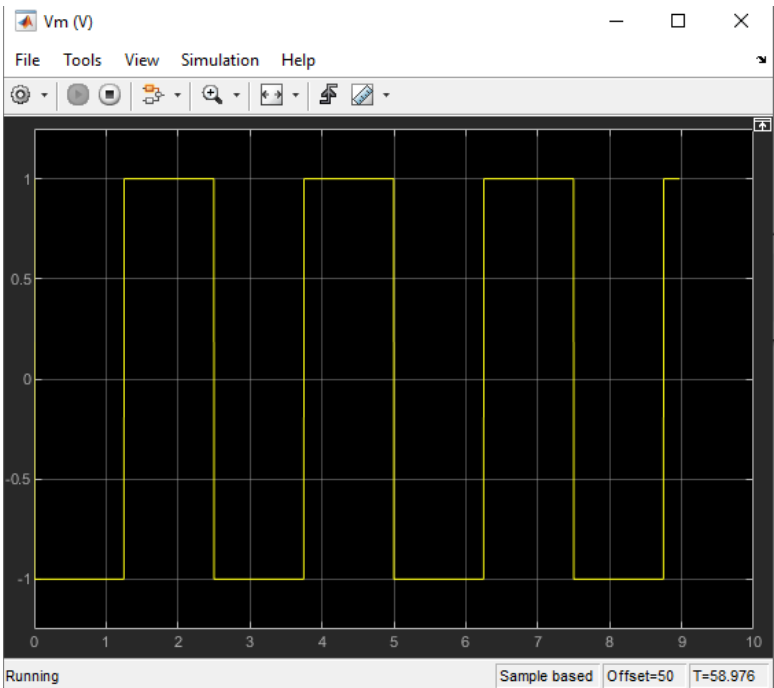
\includegraphics[width=\textwidth]{Figures/square_wave_input.png}
        \caption{Square Wave Input}
        \label{fig:my_label}
    \end{subfigure}
    \begin{subfigure}[t]{0.4\textwidth}
        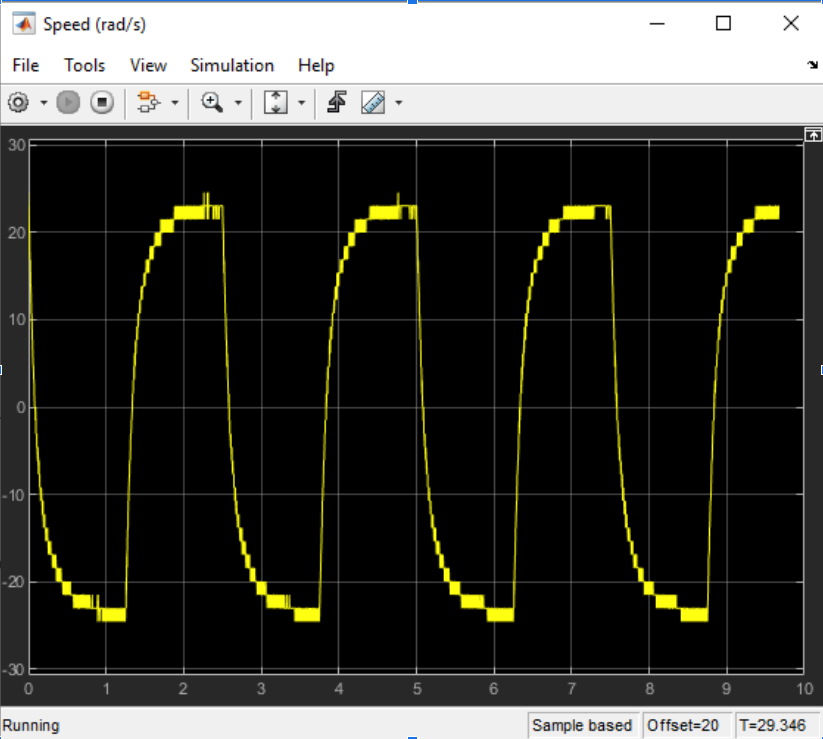
\includegraphics[width=\textwidth]{Figures/square_wave_velocity_no_filter.png}
        \caption{Response angular velocity (rad/s) with no filter}
        \label{fig:my_label}
    \end{subfigure}
    \caption{Square Wave Input and Response}
\end{figure*}

\subsection*{5.}
The encoder uses discrete pulses to measure the angle of the disc. When taking the derivative of these 
incremental (step-like) measurements, high frequencies are introduced. This is because the derivative 
of a step function is a dirac delta, which introduces high frequencies. These high frequency oscillations
appear as noise in the angular velocity signal.

The step-like nature of the encode can be seen in Fig. \ref{fig:angular_position_no_filter}. 
\begin{figure}[h]
    \centering
    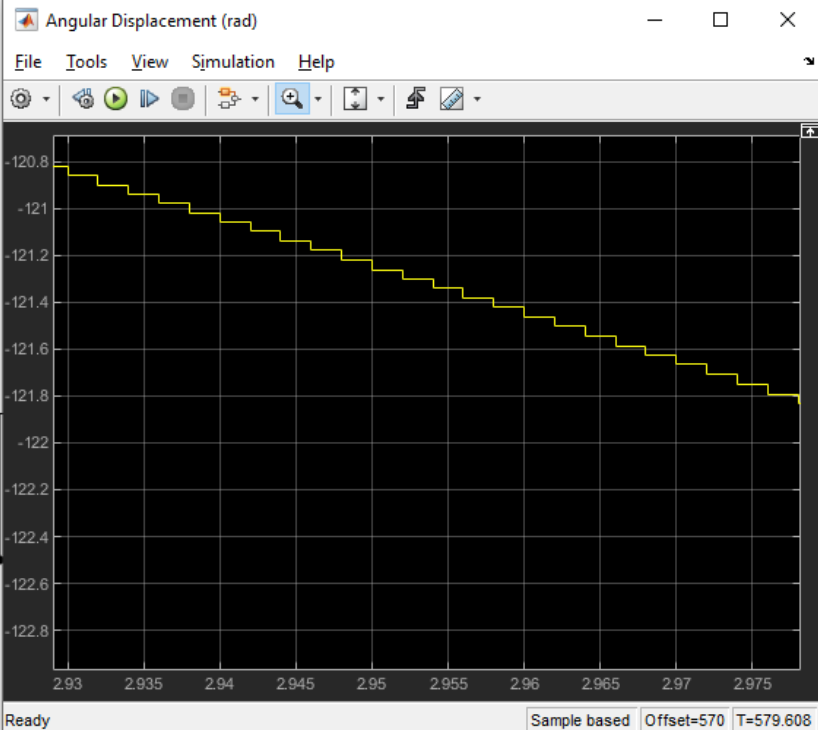
\includegraphics[width=0.5\textwidth]{Figures/square_wave_angular_displacement.png}
    \caption{Angular Position (rad) with no filter}
    \label{fig:angular_position_no_filter}
\end{figure}

\subsection*{6.}
A \texttt{Transfer Fcn} block with \texttt{num:[100]} and \texttt{den:[1 100]} was used.

\subsection*{7.}
Yes, it looks noisy still. Much of the perturbations have been removed, but there are still some.
\begin{figure}[h]
    \centering
    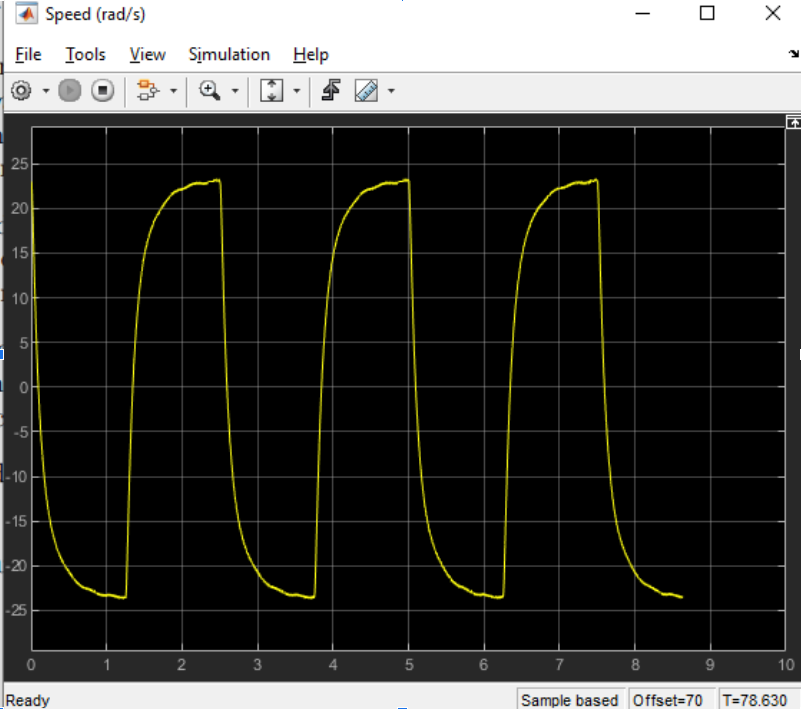
\includegraphics[width=0.5\textwidth]{Figures/square_wave_velocity_100_rad_s_filter.png}
    \caption{Response angular velocity (rad/s) with 100 rad/s filter}
    \label{fig:100_rad_s_filter}
\end{figure}

\subsection*{8.}
% Set the cut-off frequency, ωf , to 5 rad/s, then to 200 rad/s. Comment on how the angular
% velocity signal looks in each of these cases. Note: you can change the parameters of the
% transfer function block while the code is runnin

For $\omega_f = 5$ rad/s, the signal is quite clean and smooth as seen in Fig. \ref{fig:5_rad_s_filter}.

For $\omega_f = 200$ rad/s, the signal is cleaner than unfiltered, but still quite noisy as seen in Fig. \ref{fig:200_rad_s_filter}.

\begin{figure*}[h]
    \centering
    \begin{subfigure}[t]{0.4\textwidth}
        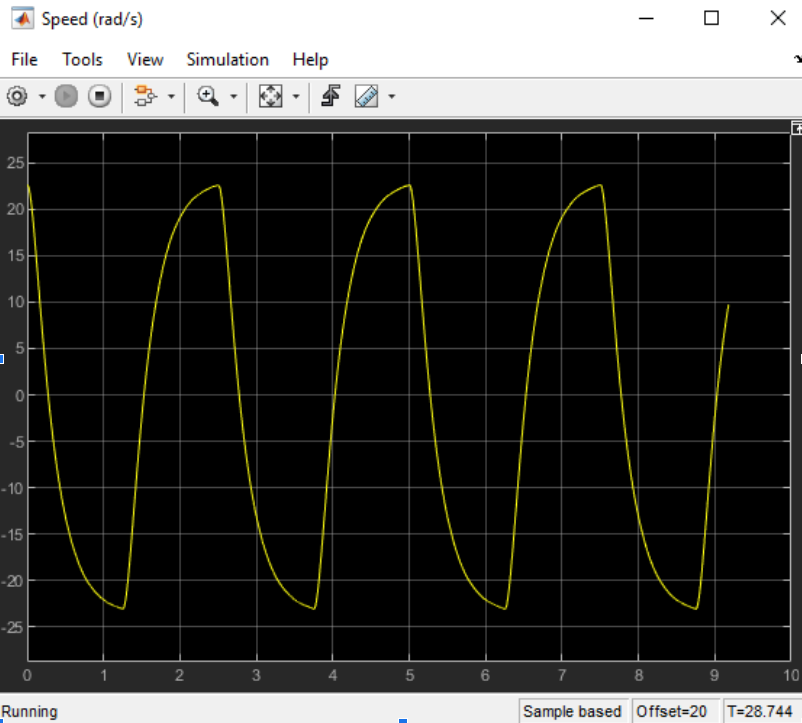
\includegraphics[width=\textwidth]{Figures/square_wave_velocity_5_rad_s_filter.png}
        \caption{Response angular velocity (rad/s) with 5 rad/s filter}
        \label{fig:5_rad_s_filter}
    \end{subfigure}
    \begin{subfigure}[t]{0.4\textwidth}
        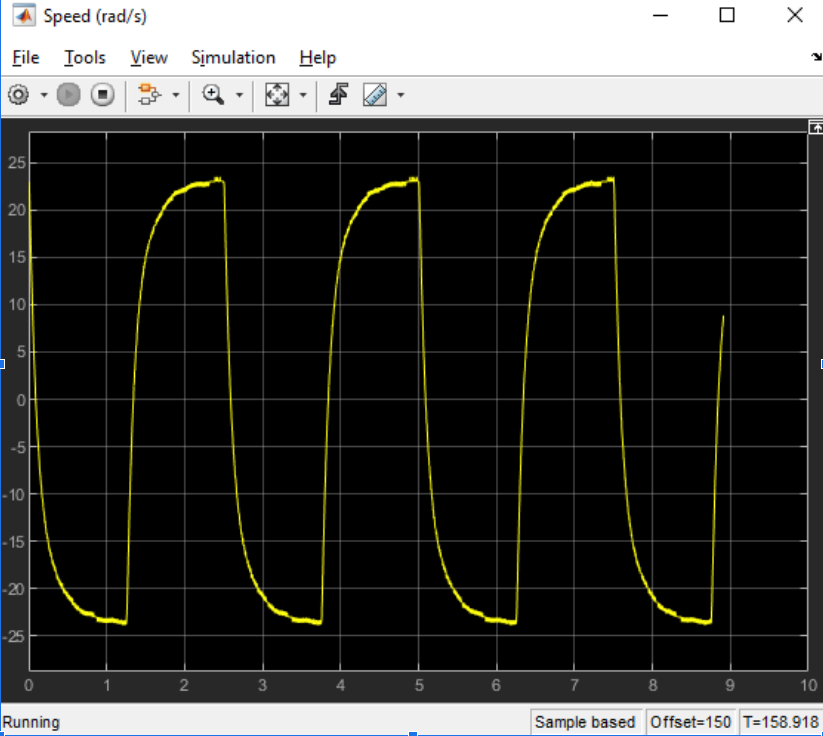
\includegraphics[width=\textwidth]{Figures/square_wave_velocity_200_rad_s_filter.png}
        \caption{Response angular velocity (rad/s) with 200 rad/s filter}
        \label{fig:200_rad_s_filter}
    \end{subfigure}
    \caption{Square Wave Input and Response with Different Filters}
\end{figure*}
\phantom{a}
\end{document}